\subsection{بخش ج}
در این بخش محدود کننده شتاب ورودی به سیستم اضافه شده و نتایج آن مقایسه شده است.

\begin{table}[H]
	\caption{مقایسه فاصله ازدست‌دهی در حضور و عدم حضور محدود کننده}
	\centering
	\begin{tabular}{cc}
		\hline
		\lr{Miss Distance (m)} &  \lr{Saturation Mode} \\
		\hline
 \lr{0.6034} & 	\lr{Off} \\
 \lr{5.1746} &	\lr{On}   \\ 
		\hline
	\end{tabular}
\end{table}


\begin{figure}[H]
	\centering
	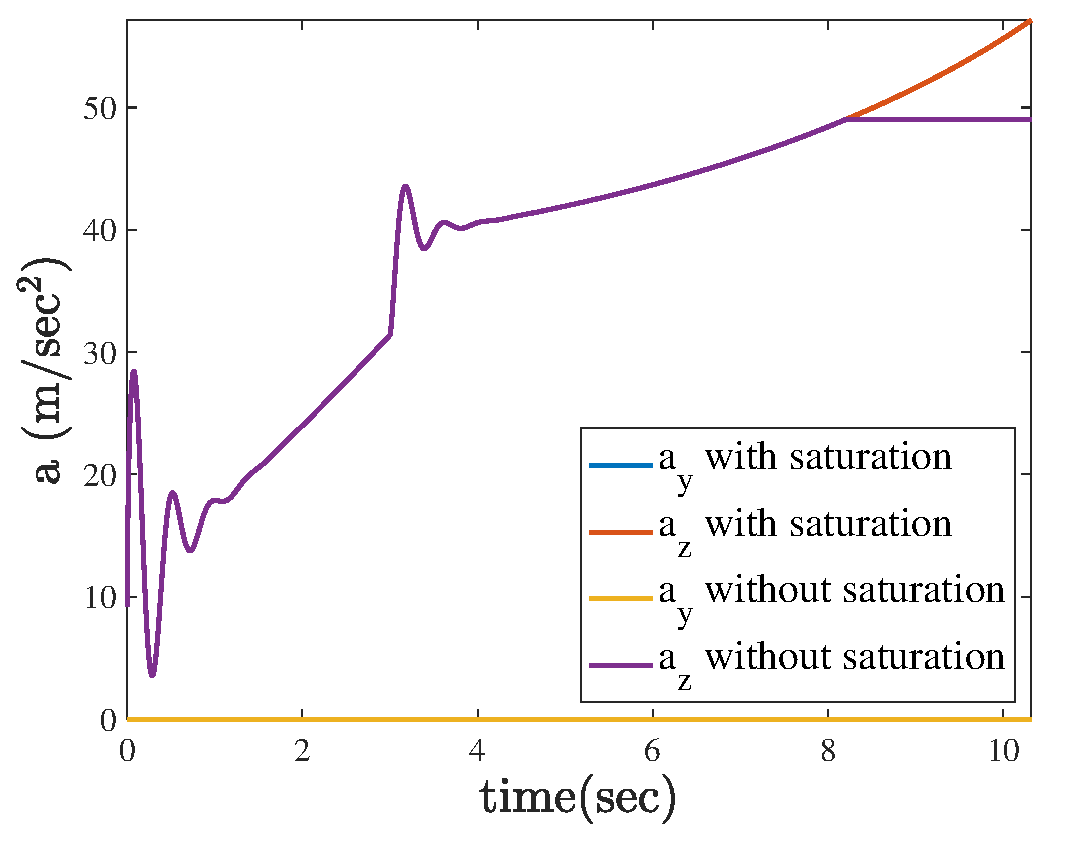
\includegraphics[width=.75\linewidth]{../Figure/f/command}
	\caption{مقایسه فرمان موشک در حضور و عدم حضور  محدود کننده در هدایت خط دید پایه همراه با مشتق‌گیر}
\end{figure}

\begin{figure}[H]
	\centering
	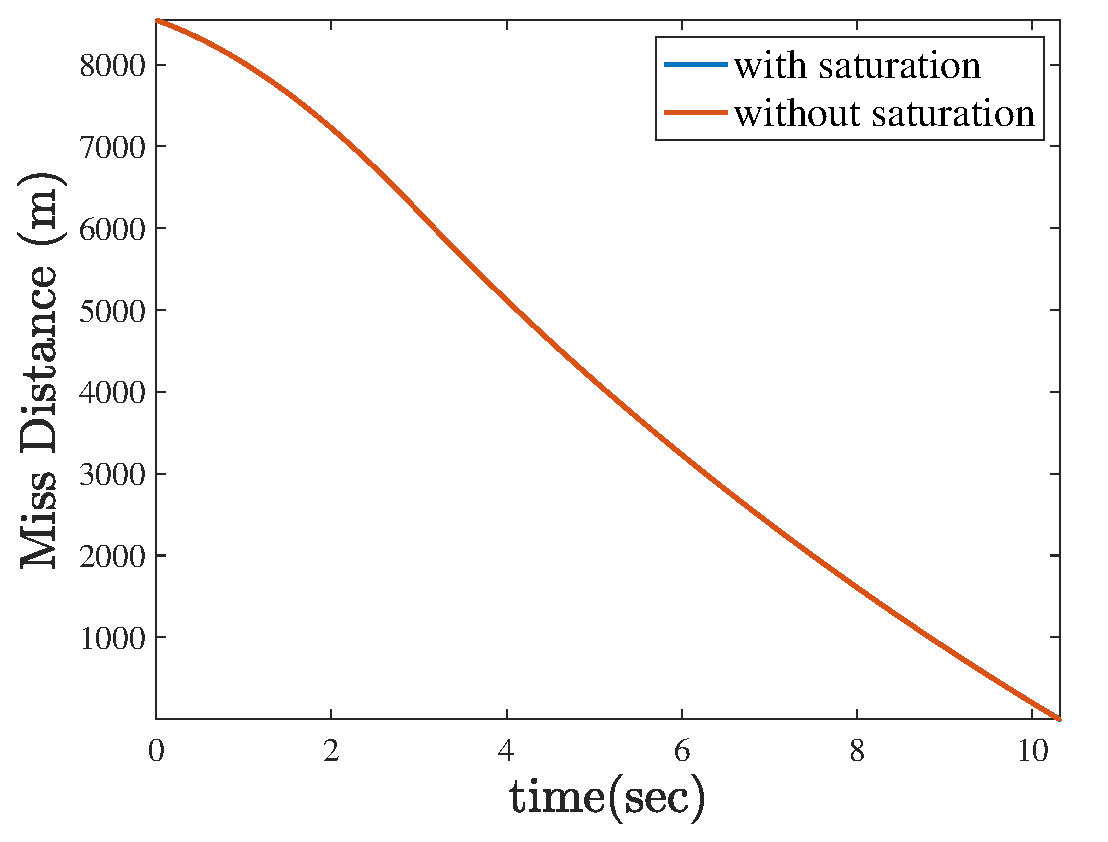
\includegraphics[width=.75\linewidth]{../Figure/f/miss_distance}
	\caption{مقایسه فاصله ازدست‌دهی موشک در حضور و عدم حضور  محدود کننده در هدایت خط دید پایه همراه با مشتق‌گیر}
\end{figure}

